\documentclass[12pt,a4paper]{article}
\usepackage{ctex}
\usepackage{listings}
\usepackage{xcolor}
\usepackage{fancyhdr}
\usepackage{graphicx}
\usepackage{geometry}  
\usepackage{booktabs}
\geometry{a4paper,left=10mm,right=10mm,top=25mm,bottom=25mm}
\pagestyle{fancy}
\rhead{Mingchen Liu}
\lstset{
    %backgroundcolor=\color{red!50!green!50!blue!50},%代码块背景色为浅灰色
    rulesepcolor= \color{gray}, %代码块边框颜色
    breaklines=true,  %代码过长则换行
    numbers=left, %行号在左侧显示
    numberstyle= \small,%行号字体
    %keywordstyle= \color{red},%关键字颜色
    commentstyle=\color{gray}, %注释颜色
    frame=shadowbox%用方框框住代码块
    }

% Title
\title{《ERP与供应链》课程作业}
\author{刘铭宸\\软件工程2003班\\U202010783}
\date{\today}
 
\begin{document}

\begin{titlepage}
\maketitle
\end{titlepage}

\tableofcontents

\newpage
\section{问题一}
以FS食品公司为应用背景,开发一个库存管理系统,
管理FS公司的原材料库存和产成品库存。
在如下功能设计(图1)和ER图(图2)设计的基础上,详细定义ER模型,
并进一步从中提取能够支持库存量动态分析的数据,
写出提取数据的sql语句。
\begin{figure}[h]
    \centering
    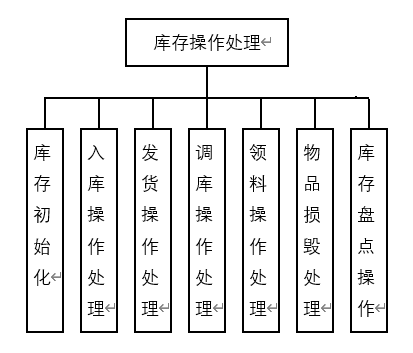
\includegraphics[scale=0.6]{fig1.png}
    \caption{库存管理系统功能设计}
    \label{fig:1}
\end{figure}
\begin{figure}[h]
    \centering
    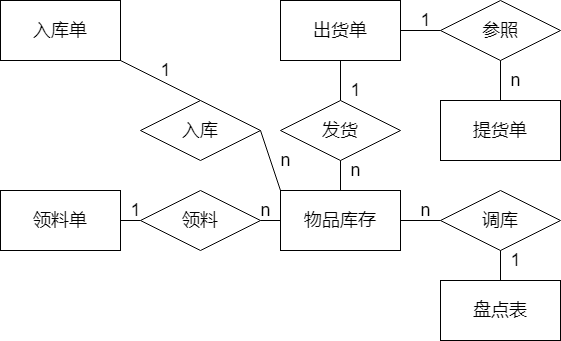
\includegraphics[scale=0.6]{fig2.png}
    \caption{库存管理系统ER图}
    \label{fig:2}
\end{figure}

\subsection{ER模型}
根据题目对库存管理系统的功能设计要求并参照ERP设计图表,对该库存管理系统的ER图进行了扩充,
结果如图3所示。
\begin{figure}[h]
    \centering
    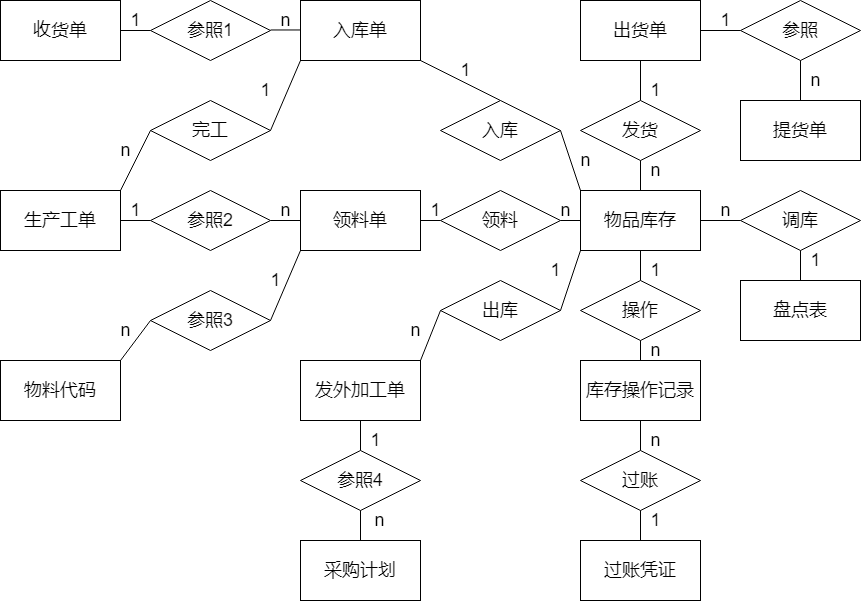
\includegraphics[scale=0.5]{fig3.png}
    \caption{详细ER图}
    \label{fig:3}
\end{figure}

对ER模型的详细定义如下列表所示。
\begin{table}[h]
    \centering
    \begin{tabular}{|c|c|c|c|c|} 
     \hline
     \multicolumn{5}{|c|}{物品库存表(Inventory)}\\
     \hline
     Field & Length & Type & Description & PrimKey/ForeKey\\\hline
        ItemID      & 10     & VARCHAR & 物品编号          & PrimKey         \\ \hline
        ItemName    & 50     & VARCHAR & 物品名称          &                 \\ \hline
        Category    & 20     & VARCHAR & 物品分类          &                 \\ \hline
        Quantity    & 10     & INT     & 库存数量          &                 \\ \hline
        Unit        & 10     & VARCHAR & 单位              &                 \\ \hline
        LastUpdate  & -      & DATETIME& 最后更新时间      &                 \\ \hline   
    \end{tabular}
    \label{table:1}
\end{table}

\begin{table}[h]
    \centering
    \begin{tabular}{|c|c|c|c|c|} 
     \hline
     \multicolumn{5}{|c|}{盘点表(InventoryCheck)}\\
     \hline
        Field       & Length & Type    & Description      & PrimKey/ForeKey \\ \hline
        CheckID     & 10     & VARCHAR & 盘点编号          & PrimKey         \\ \hline
        ItemID      & 10     & VARCHAR & 物品编号          & ForeKey         \\ \hline
        CheckDate   & -      & DATE    & 盘点日期          &                 \\ \hline
        Quantity    & 10     & INT     & 盘点数量          &                 \\ \hline
        Operator    & 20     & VARCHAR & 操作员            &                 \\ \hline
    \end{tabular}
    \label{table:2}
\end{table}


\begin{table}[h]
    \centering
    \begin{tabular}{|c|c|c|c|c|} 
     \hline
     \multicolumn{5}{|c|}{入库单(InboundOrder)}\\
        \hline
        Field       & Length & Type    & Description      & PrimKey/ForeKey \\ \hline
        OrderID     & 10     & VARCHAR & 入库单编号        & PrimKey         \\ \hline
        ItemID      & 10     & VARCHAR & 物品编号          & ForeKey         \\ \hline
        InboundDate & -      & DATE    & 入库日期          &                 \\ \hline
        Quantity    & 10     & INT     & 入库数量          &                 \\ \hline
        Operator    & 20     & VARCHAR & 操作员            &                 \\ \hline
        \end{tabular}
    \label{table:3}
\end{table}

\begin{table}[h]
    \centering
    \begin{tabular}{|c|c|c|c|c|} 
     \hline
     \multicolumn{5}{|c|}{领料单(PickList)}\\
        \hline
            Field       & Length & Type    & Description      & PrimKey/ForeKey \\ \hline
            PickID      & 10     & VARCHAR & 领料单编号        & PrimKey         \\ \hline
            ItemID      & 10     & VARCHAR & 物品编号          & ForeKey         \\ \hline
            PickDate    & -      & DATE    & 领料日期          &                 \\ \hline
            Quantity    & 10     & INT     & 领料数量          &                 \\ \hline
            Operator    & 20     & VARCHAR & 操作员            &                 \\ \hline
            \end{tabular}
    \label{table:4}
\end{table}

\begin{table}[h]
    \centering
    \begin{tabular}{|c|c|c|c|c|} 
     \hline
     \multicolumn{5}{|c|}{出货单(OutboundOrder)}\\
        \hline
            Field       & Length & Type    & Description      & PrimKey/ForeKey \\ \hline
            OrderID     & 10     & VARCHAR & 出货单编号        & PrimKey \\ \hline
            ItemID & 10 & VARCHAR & 物品编号 & ForeKey \\ \hline
            OutboundDate& - & DATE & 出货日期 & \\ \hline
            Quantity & 10 & INT & 出货数量 & \\ \hline
            Operator & 20 & VARCHAR & 操作员 & \\ \hline
            \end{tabular}
    \label{table:5}
\end{table}

\begin{table}[ht]
    \centering
    \begin{tabular}{|c|c|c|c|c|} 
     \hline
     \multicolumn{5}{|c|}{提货单(PickUpOrder)}\\
        \hline
            Field       & Length & Type    & Description      & PrimKey/ForeKey \\ \hline
            PickUpID & 10 & VARCHAR & 提货单编号 & PrimKey \\ \hline
ItemID & 10 & VARCHAR & 物品编号 & ForeKey \\ \hline
PickUpDate & - & DATE & 提货日期 & \\ \hline
Quantity & 10 & INT & 提货数量 & \\ \hline
Customer & 50 & VARCHAR & 客户名称 & \\ \hline
Operator & 20 & VARCHAR & 操作员 & \\ \hline
            \end{tabular}
    \label{table:6}
\end{table}

\begin{table}[h]
    \centering
    \begin{tabular}{|c|c|c|c|c|} 
     \hline
     \multicolumn{5}{|c|}{生产工单表(ProductionOrder)}\\
        \hline
            Field             & Length & Type    & Description        & PrimKey/ForeKey \\ \hline
            ProductionOrderID & 10     & VARCHAR & 生产工单编号        & PrimKey         \\ \hline
            ItemID            & 10     & VARCHAR & 物品编号            & ForeKey         \\ \hline
            StartDate         & -      & DATE    & 开始生产日期        &                 \\ \hline
            EndDate           & -      & DATE    & 结束生产日期        &                 \\ \hline
            Quantity          & 10     & INT     & 生产数量            &                 \\ \hline
            Status            & 20     & VARCHAR & 生产状态            &                 \\ \hline
            Operator          & 20     & VARCHAR & 操作员              &                 \\ \hline
            \end{tabular}
    \label{table:7}
\end{table}

\clearpage
\subsection{提取数据的sql语句}
为了支持库存量的动态分析,我们可以提取各个表中与库存变动相关的数据。以下是提取数据的SQL语句:

\textbf{查询当前库存总量}:
\begin{lstlisting}[language={SQL}]
    SELECT ItemID, ItemName, Category, Quantity, Unit, LastUpdate
    FROM Inventory; 
\end{lstlisting}

\textbf{查询某个时间段内的入库数量}:
\begin{lstlisting}[language={SQL}]
    SELECT ItemID, SUM(Quantity) AS InboundTotal
    FROM InboundOrder
    WHERE InboundDate BETWEEN '开始日期' AND '结束日期'
    GROUP BY ItemID;
\end{lstlisting}

\textbf{查询某个时间段内的领料数量}:
\begin{lstlisting}[language={SQL}]
    SELECT ItemID, SUM(Quantity) AS PickTotal
    FROM PickList
    WHERE PickDate BETWEEN '开始日期' AND '结束日期'
    GROUP BY ItemID;    
\end{lstlisting}

\textbf{查询某个时间段内的出货数量}:
\begin{lstlisting}[language={SQL}]
    SELECT ItemID, SUM(Quantity) AS OutboundTotal
    FROM OutboundOrder
    WHERE OutboundDate BETWEEN '开始日期' AND '结束日期'
    GROUP BY ItemID;       
\end{lstlisting}

\textbf{查询某个时间段内库存变动情况(合并入库、领料、出货、提货数量)}:
\begin{lstlisting}[language={SQL}]
    WITH InboundTotal AS (
        SELECT ItemID, SUM(Quantity) AS InQty
        FROM InboundOrder
        WHERE InboundDate BETWEEN '开始日期' AND '结束日期'
        GROUP BY ItemID
    ),
    PickTotal AS (
        SELECT ItemID, SUM(Quantity) AS PickQty
        FROM PickList
        WHERE PickDate BETWEEN '开始日期' AND '结束日期'
        GROUP BY ItemID
    ),
    OutboundTotal AS (
        SELECT ItemID, SUM(Quantity) AS OutQty
        FROM OutboundOrder
        WHERE OutboundDate BETWEEN '开始日期' AND '结束日期'
        GROUP BY ItemID
    ),
    PickUpTotal AS (
        SELECT ItemID, SUM(Quantity) AS PickUpQty
        FROM PickUpOrder
        WHERE PickUpDate BETWEEN '开始日期' AND '结束日期'
        GROUP BY ItemID
    )
    SELECT i.ItemID, i.ItemName, i.Category, i.Unit,
        COALESCE(it.InQty, 0) AS InboundQty,
        COALESCE(pt.PickQty, 0) AS PickQty,
        COALESCE(ot.OutQty, 0) AS OutboundQty,
        COALESCE(pu.PickUpQty, 0) AS PickUpQty
    FROM Inventory i
    LEFT JOIN InboundTotal it ON i.ItemID = it.ItemID
    LEFT JOIN PickTotal pt ON i.ItemID = pt.ItemID
    LEFT JOIN OutboundTotal ot ON i.ItemID = ot.ItemID
    LEFT JOIN PickUpTotal pu ON i.ItemID = pu.ItemID;          
\end{lstlisting}

\clearpage
\section{问题二}
以附件文件“库存数据.xlsx”excel表格文档数据为ABCDEF共6种物品的每小时库存量值,
进行统计分析和数据挖掘,分析这6种物品的库存量变化规律,结合库存管理的原理,
提出对这6种物品进行库存管理的改进计划。
\subsection{数据分析}
\subsubsection{拟合曲线}
首先对六种物品的库存量随时间变化趋势进行了分析,如图4所示。
\begin{figure}[h]
    \centering
    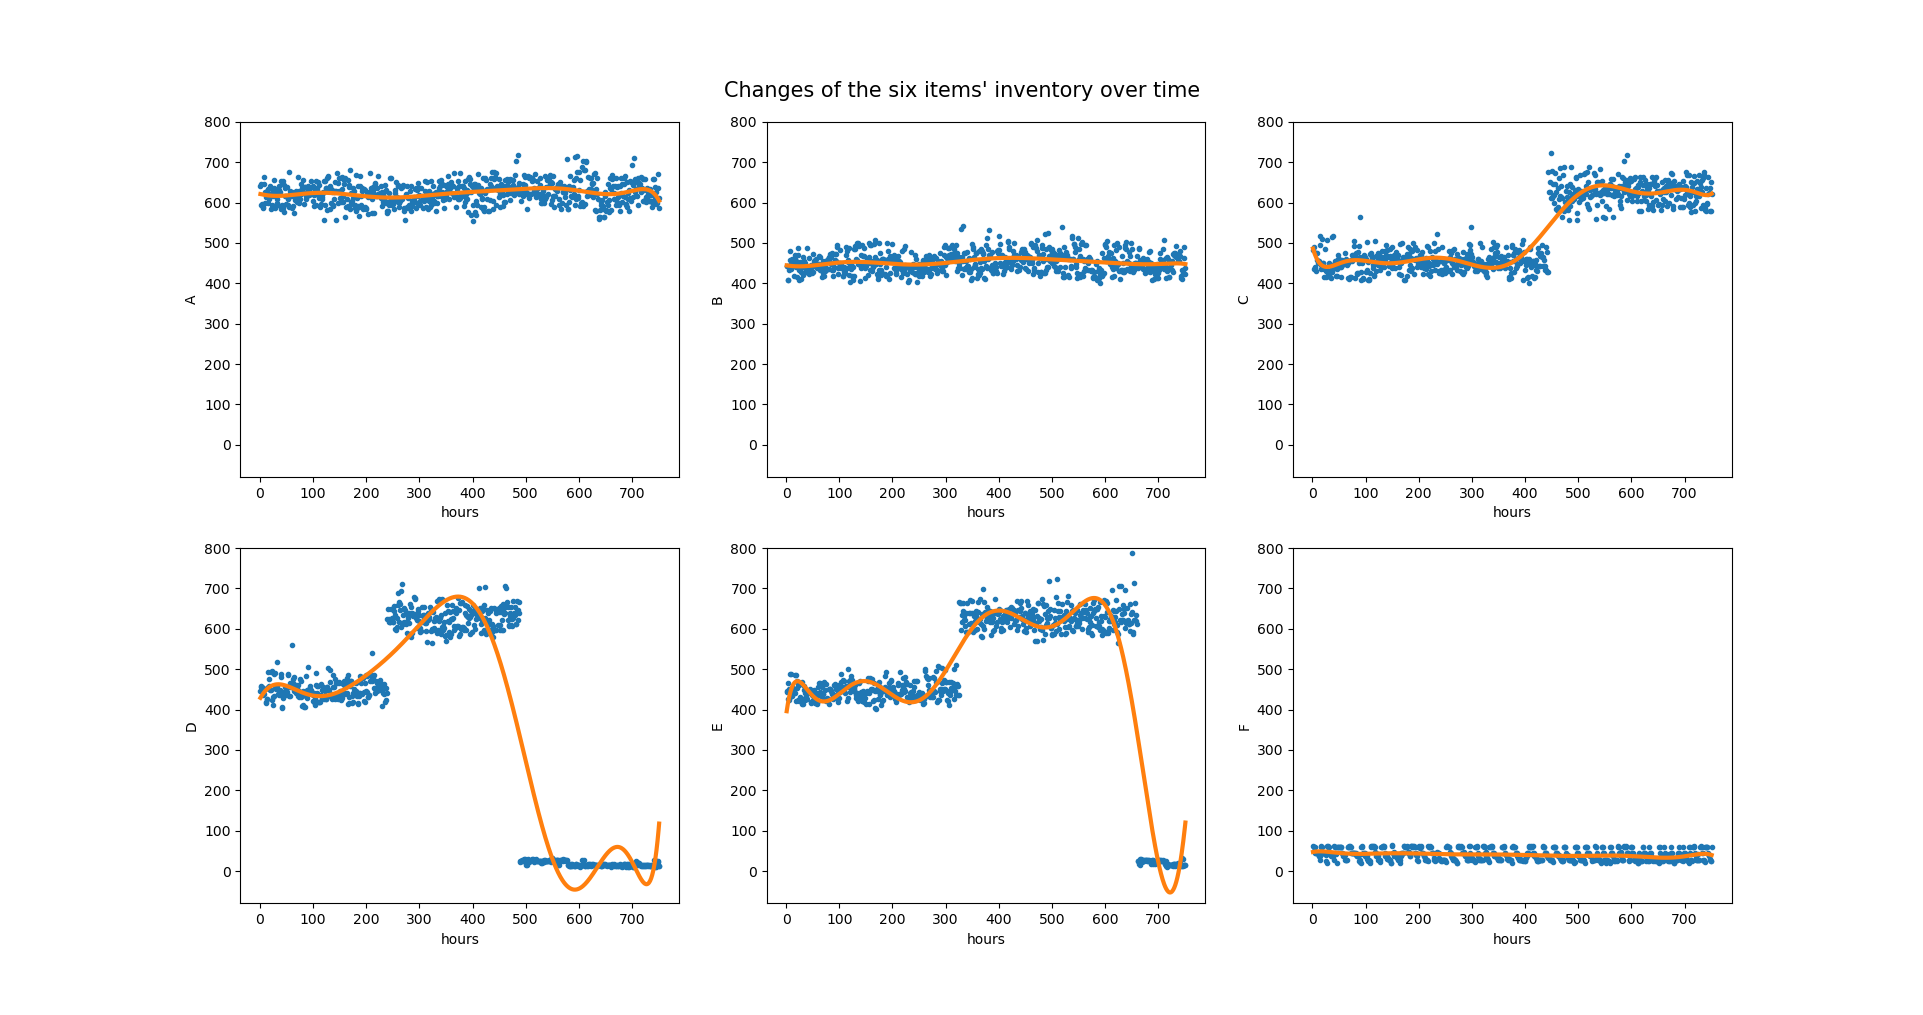
\includegraphics[scale=0.4]{fig4.png}
    \caption{六种物品的库存量随时间变化趋势}
    \label{fig:4}
\end{figure}

可以看出,物品A、物品B和物品F在这751个小时的库存量变化较少,曲线较为平缓,其中物品A和B的库存量一直维持在较高水平,物品F的库存量一直较少;
物品D和物品E的库存量存在较大的波动,随时间先增加后大量减少;物品C的库存量变化相对较小。

\subsubsection{概率分布}
六种物品的库存量的分布直方图与密度曲线如图5所示。
\begin{figure}[h]
    \centering
    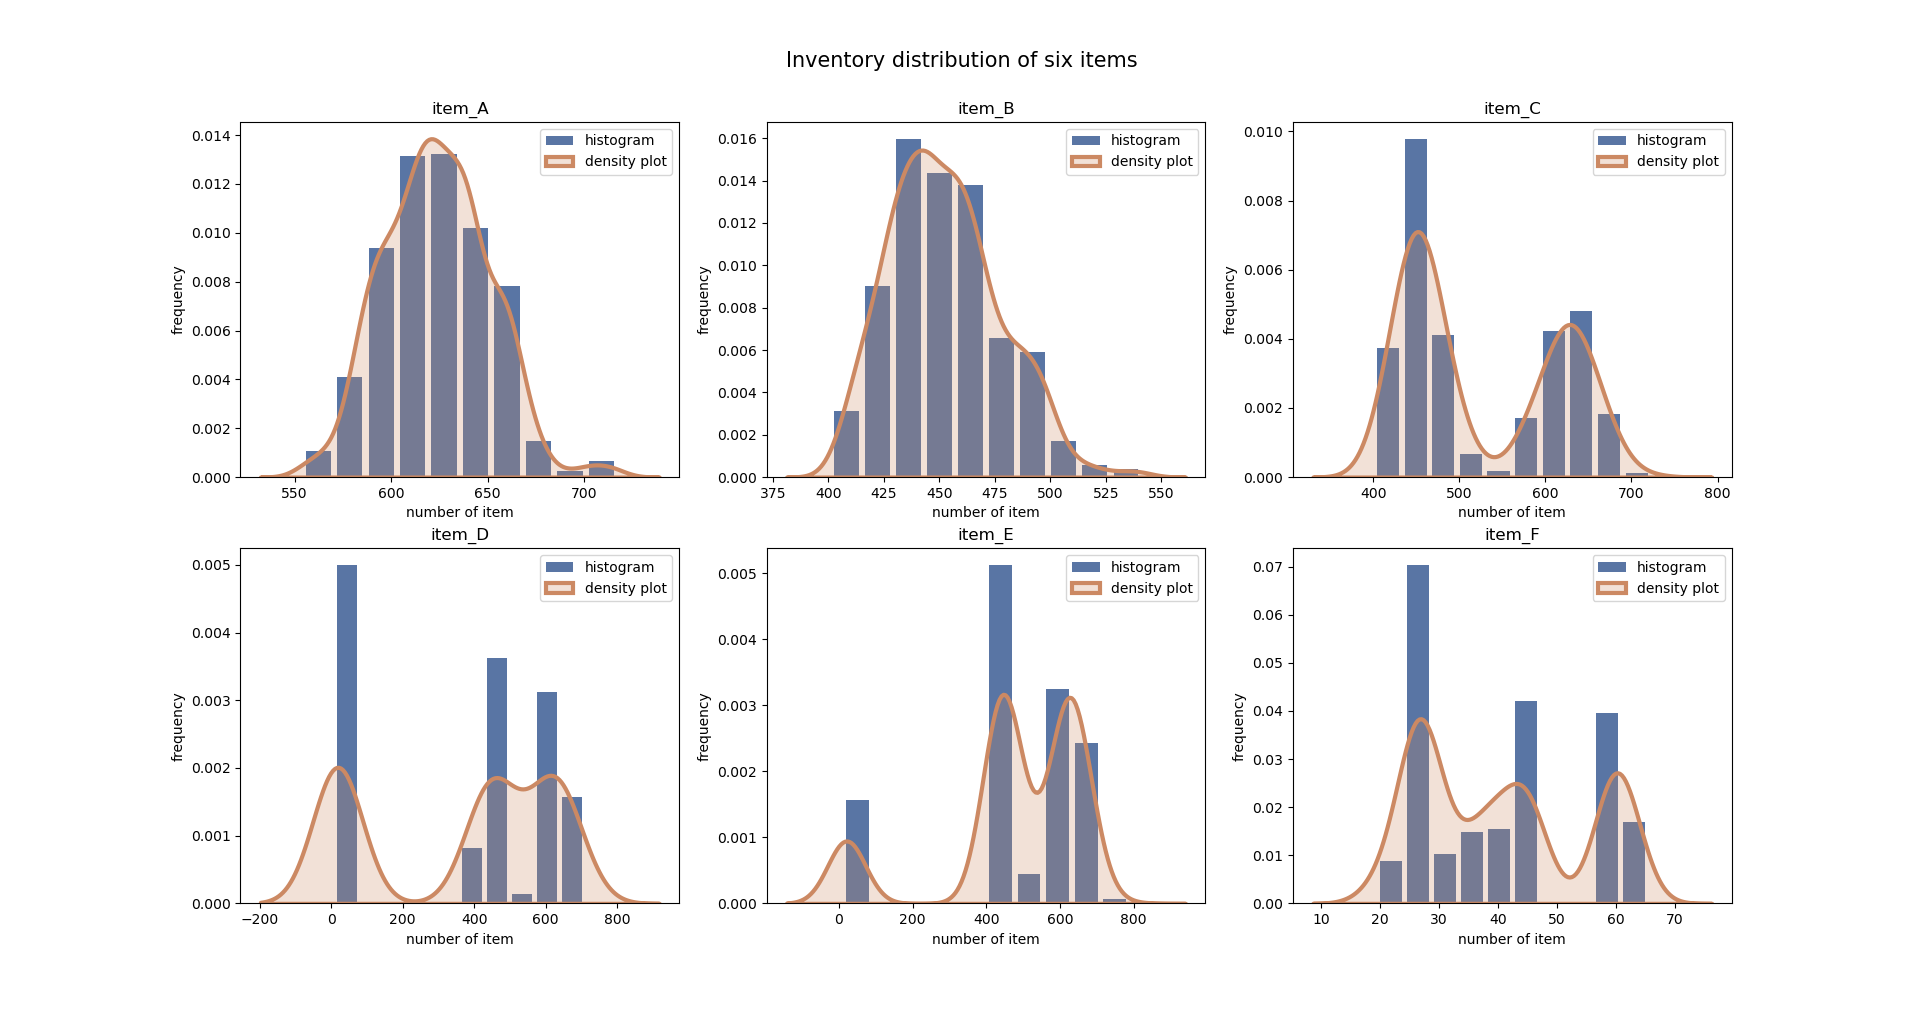
\includegraphics[scale=0.4]{fig5.png}
    \caption{六种物品的库存量的分布直方图与密度曲线}
    \label{fig:5}
\end{figure}

可以看到,物品A和物品B的库存量比较符合正态分布,说明其变化量相对均匀,起伏较小;而物品C、D、E的分布较为分散,
说明在这一时间段中库存量的变化率相对较大。

\subsubsection{统计规律}
六种物品的库存量的统计数据如表2所示。
\begin{table}[ht]
    \centering
    \setlength{\tabcolsep}{7mm}{
    \begin{tabular}{ccccccc}
    \toprule
     & A & B & C & D & E & F \\
    \midrule
    mean & 623.66 & 452.20 & 524.86 & 357.83 & 476.76 & 40.37 \\
    std & 27.25 &  24.78 &  89.25 & 260.20 & 191.03 & 13.68 \\
    min & 554 & 401 & 401 & 9.5 & 11 & 19.5 \\
    max & 717 & 541 & 722 & 710 & 788 & 65.3 \\
    \bottomrule
    \end{tabular}}
    \caption{库存量统计表}
    \label{table: 2}
\end{table}

上表列出了这六种物品库存量的平均值、标准差、最小值和最大值,从中可以更加直观地看出其库存量随时间的变化分布。
物品A、B变化较小,物品C、D、E变化较大,物品F虽然变化很小,但其库存量一直维持在较低水平。

\subsection{聚类分析}
ABC库存控制法是根据库存物品的价格来划分物品的重要程度,以分别采取不同的管理措施。但由于在库存数据中仅提供了六种库存物品
的库存量随时间(小时)的变化情况,故采用聚类方法以751个小时对应的库存量的值为根据对这六种物品进行分类。

\subsubsection{k-means}
首先对库存数据进行预处理,去除掉几个较为明显的脏数据,如删除表格中库存量属性不是数字的分量;将读入的表格数据进行转置,
使每种物品的在751个小时中的库存量成为一个数据点(751维的向量)。接着人为选择聚类数量,在对原始数据进行初步分析后(见2.1),
可以发现按照其库存量随时间分布曲线的相似度大致可以分为3类,故将聚类数量设为3。

之后使用k-means方法对这6个751维的向量进行聚类,选择k-means++作为初始化中心点的方法,最大迭代次数设置为300,并用生成的k-means模型
对数据进行聚类。

最后,由于数据维数过高(751维),所以使用主成分分析(PCA)的方法对数据进行降维以便于可视化。PCA将数据降为两维,
第一个主成分(即第一维)是数据中最大方差的方向,而第二个主成分(第二维)是与第一个主成分正交且具有次大方差的方向。这样,PCA 可以保留原始数据中尽可能多的信息,同时减少数据的维度。聚类结果如图6所示。
\begin{figure}[h]
    \centering
    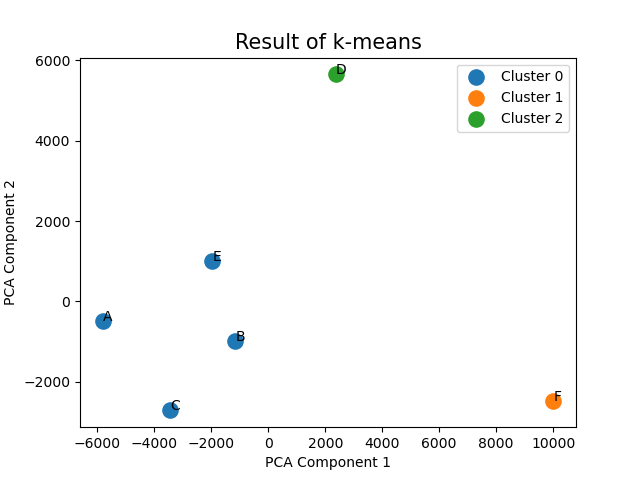
\includegraphics[scale=0.9]{fig6.png}
    \caption{k-means聚类结果}
    \label{fig:6}
\end{figure}

如图所示,k-means聚类方法将这六种物品分为了3类,分别为$\{A, B, C, E\}$、$\{D\}$和$\{F\}$。

\subsubsection{DBSCAN}
为了验证聚类方法对物品分类的可靠性,我使用了DBSCAN聚类方法(Density-Based Spatial Clustering of Applications with Noise)
来解决这一问题。与k-means不同,DBSCAN是一种基于密度的聚类算法,可以找到任意形状的聚类,并识别噪声数据点。DBSCAN 不需要预先设定聚类数量,但需要设置密度半径和最小数据点数作为参数。

计算过程与k-means类似,设定合适的密度半径使这六个物品被聚类为三类。结果如图7所示。
\begin{figure}[ht]
    \centering
    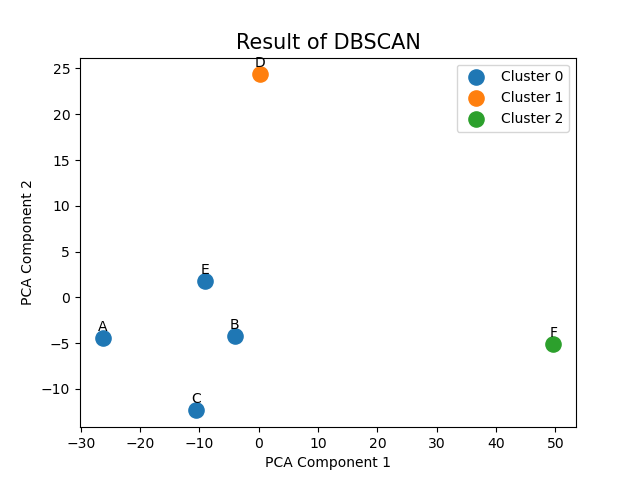
\includegraphics[scale=0.9]{fig7.png}
    \caption{DBSCAN聚类结果}
    \label{fig:7}
\end{figure}

如图所示,DBSCAN聚类方法将这六种物品分为了与k-means方法同样的三类,证明聚类分析得到的结果可靠性较高。

\subsection{库存管理的改进计划}
在库存管理中,安全库存和储备库存是两个重要概念。
安全库存是为了应对供应链不确定性而设置的额外库存,以防止缺货。
储备库存是在预期需求高峰或供应链中断期间使用的额外库存。
结合六种物品的库存统计数据的分析,我们可以提出以下针对各物品的库存管理改进计划:

\textbf{物品A}:A物品的库存波动相对较小。可以将安全库存设置为一个较小的值(例如,标准差的 1 倍)。另外,可以适当减少最大库存量以降低库存成本。

\textbf{物品B}:B物品的库存波动也较小。与A物品类似,可以将安全库存设置为标准差的1倍,并适当调整最大库存量以降低库存成本。

\textbf{物品C}:C物品的库存波动较大。为防止缺货,建议将安全库存设置为标准差的1.5倍。同时,需要密切关注库存水平,以应对可能的需求波动。

\textbf{物品D}:D物品的库存波动非常大。为确保供应稳定,建议将安全库存设置为标准差的 2 倍。此外,需要加强对供应链的监控,以减少库存波动并确保及时供应。

\textbf{物品E}:E物品的库存波动同样很大。建议将安全库存设置为标准差的 2 倍,并密切关注库存水平。另外,与供应商合作优化供应链管理以减少库存波动。

\textbf{物品F}:F物品的库存波动较小,但相对于其平均库存量,波动仍然显著。建议将安全库存设置为标准差的 1.5 倍。另外,考虑与供应商协商更频繁的供货安排,以减少库存波动并确保库存充足。

在库存管理中,根据物品的库存波动和供应链特点,我们可以调整安全库存和储备库存水平。对于波动较大的物品(如 C、D 和 E),需要增加安全库存以防止缺货。同时,密切关注库存水平,并与供应商合作优化供应链管理以减少库存波动。
对于波动较小的物品(如 A、B 和 F),可以将安全库存设置为较低的水平,降低库存成本。另外,可以考虑与供应商协商更频繁的供货安排,以进一步减少库存波动。



\section{致谢}
感谢方少红老师的教学,希望方老师的课能越办越好!

\section{参考资料}
[1]数据集:“库存数据.xlsx".

[2]罗鸿.ERP原理$\cdot$设计$\cdot$实施(第五版)[M].北京:电子工业出版社,2020.

\section{附录}
\subsection{k-means聚类分析代码}
\begin{lstlisting}[language={python}]
    import pandas as pd
    import matplotlib.pyplot as plt
    import numpy as np
    from sklearn.cluster import KMeans
    from sklearn.decomposition import PCA

    data = pd.read_excel('库存数据.xlsx')
    # 提取物品的库存量数据,并转置,使每种物品的库存量成为一个数据点
    items_data = data.iloc[:, 1:].T
    # 选择聚类数量
    num_clusters = 3
    # 初始化 KMeans 模型
    kmeans = KMeans(n_clusters=num_clusters, random_state=0)
    # 对数据进行聚类
    kmeans.fit(items_data)
    # 得到聚类结果
    labels = kmeans.labels_
    # 使用主成分分析(PCA)降维以便于可视化
    pca = PCA(n_components=2)
    items_data_pca = pca.fit_transform(items_data)
    # 创建一个可视化图
    fig, ax = plt.subplots()
    # 为每个聚类绘制散点图
    for cluster_id in range(num_clusters):
        cluster_data = items_data_pca[labels == cluster_id]
        ax.scatter(cluster_data[:, 0], cluster_data[:, 1], label=f'Cluster {cluster_id}', s=120)
    # 设置图例和轴标签
    ax.legend()
    ax.set_xlabel('PCA Component 1')
    ax.set_ylabel('PCA Component 2')
    # 为每个数据点添加物品标签
    item_labels = ['A', 'B', 'C', 'D', 'E', 'F']
    for i, item_label in enumerate(item_labels):
        ax.annotate(item_label, (items_data_pca[i, 0], items_data_pca[i, 1]))
    plt.title("Result of k-means", fontsize=15)
    # 显示图形
    plt.show()
\end{lstlisting}

\subsection{DBSCAN聚类分析代码}
\begin{lstlisting}[language={python}]
    import pandas as pd
    import matplotlib.pyplot as plt
    import numpy as np
    from sklearn.decomposition import PCA
    from sklearn.cluster import DBSCAN
    from sklearn.preprocessing import StandardScaler

    data = pd.read_excel('库存数据.xlsx')
    # 提取物品的库存量数据,并转置,使每种物品的库存量成为一个数据点
    items_data = data.iloc[:, 1:].T
    # 对数据进行标准化
    scaler = StandardScaler()
    scaled_data = scaler.fit_transform(items_data)
    # 初始化 DBSCAN 模型
    # 调整 eps 和 min_samples 参数以获得合适的聚类结果
    dbscan = DBSCAN(eps=25, min_samples=1)
    # 对数据进行聚类
    dbscan.fit(scaled_data)
    # 得到聚类结果
    labels = dbscan.labels_
    # 使用 PCA 将数据降至二维
    pca = PCA(n_components=2)
    reduced_data = pca.fit_transform(scaled_data)
    # 创建一个可视化图
    fig, ax = plt.subplots()
    # 获取聚类数量(排除噪声点)
    num_clusters = len(set(labels)) - (1 if -1 in labels else 0)
    # 为每个聚类绘制散点图并添加物品标签
    item_labels = ['A', 'B', 'C', 'D', 'E', 'F']
    for cluster_id in range(num_clusters):
        cluster_data = reduced_data[labels == cluster_id]
        ax.scatter(cluster_data[:, 0], cluster_data[:, 1], label=f'Cluster {cluster_id}', s=120)
        for point, label in zip(cluster_data, np.array(item_labels)[labels == cluster_id]):
            ax.annotate(label, (point[0], point[1]), textcoords="offset points", xytext=(0, 5), ha='center')
    # 如果存在噪声点,将其绘制到图上并添加物品标签
    if -1 in labels:
        noise_data = reduced_data[labels == -1]
        ax.scatter(noise_data[:, 0], noise_data[:, 1], label='Noise')
        for point, label in zip(noise_data, np.array(item_labels)[labels == -1]):
            ax.annotate(label, (point[0], point[1]), textcoords="offset points", xytext=(0, 5), ha='center')
    # 设置图例和轴标签
    ax.legend()
    ax.set_xlabel('PCA Component 1')
    ax.set_ylabel('PCA Component 2')
    # 显示图形
    plt.title("Result of DBSCAN", fontsize=15)
    plt.show()
\end{lstlisting}

\end{document} 